\begin{figure}[H]
    \centering
    \begin{subfigure}{0.45\textwidth}
        \centering
        \subcaption{Some Consumers Don't Buy}
        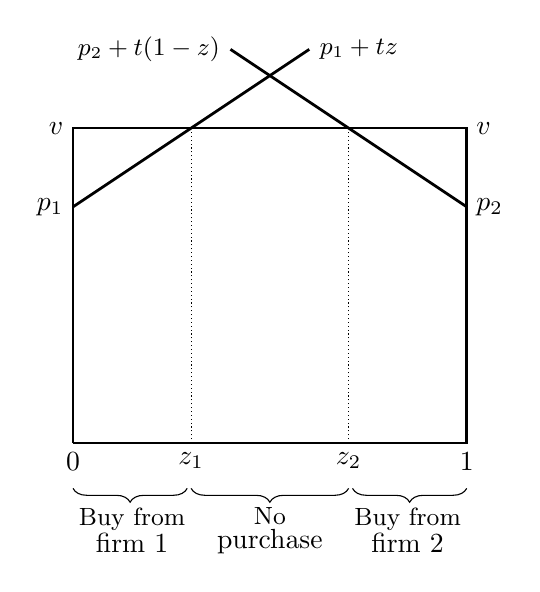
\begin{tikzpicture}[scale=1.0]
            % Outer frame
            \draw[line width=1pt] (0,0) -- (0,4) -- (5,4) -- (5,0) -- (0,0);
            % Total cost lines
            \draw[line width=1pt] (0,3) -- (3,5) node[right] {\small$p_1 + tz$};
            \draw[line width=1pt] (5,3) -- (2,5) node[left] {\small$p_2 + t(1-z)$};
            % Labels and dotted lines
            \draw[densely dotted] (1.5, 0) -- (1.5, 4);
            \draw[densely dotted] (3.5, 0) -- (3.5, 4);
            \node[below] at (0,0) {$0$};
            \node[below] at (5,0) {$1$};
            \node[below] at (1.5,0) {$z_1$};
            \node[below] at (3.5,0) {$z_2$};
            \node[left] at (0,4) {$v$};
            \node[right] at (5,4) {$v$};
            \node[left] at (0,3) {$p_1$};
            \node[right] at (5,3) {$p_2$};
            \draw [decorate, decoration = {brace, raise=5pt, amplitude=5pt}] (1.45,-0.4) --  (0,-0.4);
            \node[below, align=center, execute at begin node=\setlength{\baselineskip}{2ex}] at (0.75,-0.7) {\small Buy from \\ firm 1};
            \draw [decorate, decoration = {brace, raise=5pt, amplitude=5pt}] (3.5,-0.4) --  (1.5,-0.4);
            \node[below, align=center, execute at begin node=\setlength{\baselineskip}{2ex}] at (2.5,-0.7) {\small No \\ purchase};
            \draw [decorate, decoration = {brace, raise=5pt, amplitude=5pt}] (5,-0.4) --  (3.55,-0.4);
            \node[below, align=center, execute at begin node=\setlength{\baselineskip}{2ex}] at (4.25,-0.7) {\small Buy from \\ firm 2};
        \end{tikzpicture}
    \end{subfigure}
    \begin{subfigure}{0.53\textwidth}
        \centering
        \subcaption{All Consumers Buy}
        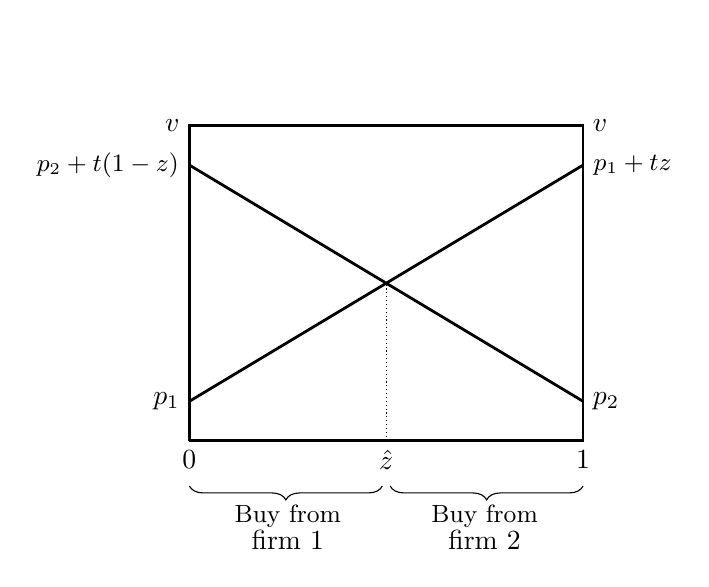
\begin{tikzpicture}[scale=1.0]
            % Outer frame
            \draw[line width=1pt] (0,0) -- (0,4) -- (5,4) -- (5,0) -- (0,0);
            % Total cost lines
            \draw[line width=1pt] (0,0.5) -- (5,3.5) node[right] {\small$p_1 + tz$};
            \draw[line width=1pt] (5,0.5) -- (0,3.5) node[left] {\small$p_2 + t(1-z)$};
            % Labels and dotted lines
            \draw[densely dotted] (2.5, 0) node[below] {$\hat{z}$} -- (2.5, 2);
            \node[below] at (0,0) {$0$};
            \node[below] at (5,0) {$1$};
            \node[left] at (0,0.5) {$p_1$};
            \node[right] at (5,0.5) {$p_2$};
            \node[left] at (0,4) {$v$};
            \node[right] at (5,4) {$v$};
            \draw [decorate, decoration = {brace, raise=5pt, amplitude=5pt}] (2.45,-0.4) --  (0,-0.4);
            \node[below, align=center, execute at begin node=\setlength{\baselineskip}{2ex}] at (1.25,-0.7) {\small Buy from \\ firm 1};
            \draw [decorate, decoration = {brace, raise=5pt, amplitude=5pt}] (5,-0.4) --  (2.55,-0.4);
            \node[below, align=center, execute at begin node=\setlength{\baselineskip}{2ex}] at (3.75,-0.7) {\small Buy from \\ firm 2};
            % The following line is used to make the subfigures placed at the same horizon.
            \node[right] at (3,5) {\color{white}\small$p_1 + tz$};
        \end{tikzpicture}
    \end{subfigure}
\end{figure}